\chapter{EpipolarNVS: leveraging on Epipolar geometry for single-image NVS} 
\label{chapter:epipolarnvs}

\ifthenelse{\boolean{skipEpipolarNVS}}{\endinput}{}

\newcommand{\tableindent}{\,\,\,\,}
\newcommand{\vt}{\mathbf{t}}

\newcommand{\std}{$\pm\,$}
\newcommand{\clf}{\textit{clf}} \newcommand{\gray}[1]{{\color{darkgray}#1}}

\chapterwithfigures{\nameref*{chapter:epipolarnvs}}
\chapterwithtables{\nameref*{chapter:epipolarnvs}}

\ifthenelse{\boolean{skipEpipolarNVS}}{\endinput}{}

\ac{NVS} can be approached from various data sources perspectives, ranging from a single image to a video sequence, with or without provided camera pose information, by leveraging 3D-based prior information, such as point clouds, or not. The most challenging scenario, which is the focus of this chapter, involves generating a novel viewpoint from a unique source image. However, in this complex case, the latest learning-based solutions often struggle to efficiently integrate the camera viewpoint transformation. Indeed, the extrinsic information is often passed as-is through a low-dimensional vector. In some cases, the camera pose is even quantized using a one-hot representation when parametrized as Euler angles. This vanilla encoding choice prevents the learned architecture from inferring novel views at any viewpoint that was not registered. 

We argue that there is a better way to encode this relative camera pose by leveraging 3D-related concepts, such as the epipolar constraint. We thus introduce in this chapter a method that encodes the viewpoint transformation as a 2D feature image. This camera encoding strategy provides the network with meaningful insights regarding how the camera has moved in space between the two views. By encoding the camera pose information as a finite number of colored epipolar lines, we demonstrate through our experiments that our strategy outperforms vanilla encoding. 

\section{Introduction}

The \ac{NVS} problem can be addressed from different perspectives, depending on available data: number of source images, geometrical priors such as depth or normal maps, 3D scene information trough point cloud, textured meshes, accurate or jittered camera poses etc. We considered in this first chapter one of the most extreme cases for the novel-view synthesis issue. Our work constrains the prediction of a novel viewpoint from a scene by solely leveraging a single source image and the corresponding camera viewpoint transformation. 

Eforts in\ac{NVS} are often oriented toward getting the most visually appealing results, mainly through \ac{NeRF}-based methods \citep{mildenhall2020nerf,wang2021neus,barron2021mip,barron2022mip}. However, only a limited number of works pursue another tricky challenge in \ac{NVS}: investigate a more efficient way to condition a single-image \ac{NVS} architecture on camera pose information. From a general perspective, associated methods often restrict the viewpoint transformation to the extrinsic matrix. Intrinsic is thus discarded since most methods for single-image \ac{NVS} ignore physical image formation properties and do not account for rendering, epipolar geometry or homography concepts. This camera pose conditioning task remains too weakly addressed in the current literature, which motivated us to tackle such an issue in an original way.

While one of the most straightforward solutions to do so consists in encoding the relative camera viewpoint transformation as a feature vector, we claim such a method is sub-optimal, supported by one of the latest state-of-the-art works in monocular depth prediction \citep{zhao2021camera}. We thus propose in this work an innovative solution to encode the camera relative transformation as a 2D feature RGB image, by leveraging epipolar constraints. The new and implicitly encoded camera viewpoint transformation has a similar spatial resolution as the source image, somehow filling the dimensional gap between pose matrices and the RGB space. The contribution we propose in this first chapter is thus three-fold: 
\begin{itemize}
	\item A strategy to encode the camera pose transformation into an implicit feature image builds upon epipolar geometry considerations. 
	\item A neural network architecture that account for this camera viewpoint transformation encoding. 
	\item A spectral loss function that focus onto image highest frequencies to better synthesize complex details.
\end{itemize}

\section{Related work}

\noindent\textbf{Novel view synthesis.} Since modalities involved in \ac{NVS} are diverse (\textit{e.g} images, video sequence, 3D point clouds,meshes, depth or disparity maps, camera poses), various approaches have been explored to adress the novel viewpoint generation challenge. One of the latest trends leverages the power of \ac{NeRF} \citep{mildenhall2020nerf} to render highly realistic scenes from unseen viewpoints \citep{wang2021neus,niemeyer2022regnerf,barron2022mip}. However, in their original formulation, these neural radiance-based  architectures overfir to a single scene and lack generalization capabilities. Recent works \citep{yu2021pixelnerf,li2021mine} have increasingly addressed this limitation by adapting NeRF-based architectures to the single-image \ac{NVS} problem. The next chapter \ref{chapter:epinerf} will also focus on how these generalizable \ac{NeRF} networks can be employed with geometric constraints to tackle this issue. While MINE \citep{li2021mine} is a \ac{MPI} based method that requires accurate ground truth disparity maps, PixelNeRF \citep{yu2021pixelnerf} uses one or multiple input views to render novel viewpoints. Another important area of \ac{NVS} research for indoor navigation uses datasets like RealEstate10K \citep{zhou2018stereo} and Matterport3D \citep{zhao2021camera}. These approaches achieve impressive results with complex architectures \citep{wiles2020synsin,rombach2021geometry,rockwell2021pixelsynth}, but they often rely on hard-to-obtain data, such as ground truth depth maps or dense 3D point clouds.. \newline

\noindent\textbf{Camera pose encoding.} Camera pose can be represented by three degrees of rotations around each world axis and three more for translation, which together define the extrinsic matrix.  Itrinsic parameters, such as focal length or sensor size could also be considered, leading to few more degrees to embed. One straightforward solution encodes viewpoint transformations by computing camera poses difference \citep{sun2018multiview}. Another approach embeds this low-dimentional camera pose information into a higher-dimentional space, as seen in \citep{kim2020novel,rombach2021geometry}. These last two methods can be further simplified using one-hot vectors for camera pose encoding. Finally, the closest work to ours regarding camera pose encoding is \citep{zhao2021camera}. It encodes the camera location (parametrized through a roll and pitch angles as well as a fixed height above a ground plane) as a 2D feature image for predicting depth maps. \newline

\noindent\textbf{Camera pose conditioning.} Extrinsic camera pose is often the only 3D prior information used to condition a neural network for generating novel viewpoints. Based on the camera pose difference $P_{diff}=P_{target}-P_{source}\in \mathbb{R}^{v}$, the authors in \citep{sun2018multiview} tiled this vector across all the pixels of the source RGB image, feeding their \ac{CNN}-based architecture with inputs sized $\mathbb{R}^{H\times W\times (3+v)}$. In contrast, \citep{kim2020novel} used a different strategy by concatenating the camera pose feature vector with the one obtained from their \ac{CNN} encoder before passing it to the decoder. 
Lastly, \citep{wiles2020synsin} designed a single-image \ac{NVS} method that extensively relies on 3D point clouds. The camera viewpoint transformation is applied within the network architecture to update the predicted point cloud before rendering. \newline

\noindent\textbf{Single-image novel view synthesis.} This framework is the most challenging one because minimal information is available during training and inference: a source image and the corresponding camera pose transformation needed to generate the target image. To the best of our knowledge, only a few recent works \citep{sun2018multiview,kim2020novel,yu2021pixelnerf} address this highly constrained setting. While \citep{sun2018multiview, kim2020novel} handle discretized camera transformation (from ShapeNet \citep{chang2015shapenet}, through a unique azimuthal angle since elevation is fixed) and continuous ones (in Synthia \citep{ros2016synthia} and KITTI \citep{geiger2012we} datasets), the pose-feature vector must be adjusted in size accordingly. This adaptability is one of the main benefits of the method we designed. Both discrete and continuous camera transformations are encoded as a featured image with the same resolution as the source image, effectively capturing the real-world transformation between the source and the target views. This property allows us to infer viewpoints, at least for discrete poses, that were not represented within the training set. \newline

\section{Method}
\subsection{Camera viewpoint transformation encoding}
\subsubsection{Epipolar geometry overview }

The general framing of our work can be considered as one of the most challenging, as generating an  image from a different camera viewpoint is only made prior to a single source image and a relative camera transformation. 

We denote the RGB source image as $I_{s} \in \mathbb{R}^{H\times W\times 3}$ and the target view, which we aim to predict, as $I_{t}$.

The pinhole camera model we consider is represented by the intrinsic matrix $K \in \mathbb{R}^{3\times3}$. The rigid motion that accounts for the relative transformation between the source and the target view consists of a rotation $R \in SO(3)$ and translation $T\in \mathbb{R}^{3\times1}$, expressed through the extrinsic parameters of each camera:

\begin{equation}
     \begin{cases}
     R = R_{t} R_{s}^{T} \\
     T = t_{t} - R t_{s}
     \end{cases}
\end{equation}

with $(R_{s},t_{s})$ and $(R_{t},t_{t})$ respectively the source and target camera extrinsics. Epipolar geometry \citep{hartley2003multiple} addresses the projective geometry that connects two camera viewpoints and has various applications such as \ac{SFM} \citep{tamaazousti2011nonlinear}. Epipolar geometry aims to describe the relationship that stands between 3D world location and 2D pixel coordinates, given a stereo pair of cameras and their corresponding poses. The fundamental matrix F is a $3\times3$ matrix that entirely describes such 3D/2D mapping: 
\begin{equation}
    \mathbf{F} = K^{-T} [T]_{X} R  K^{-1}
\end{equation}

with $[.]_{X}$ the skew-symmetric matrix representation of any one-dimensional vector. Given a pixel location\footnote{Homogeneous coordinates are implicitly used here but omitted for clarity reason} $p_{s}\in I_{s}$, such fundamental matrix $\mathbf{F} \in \mathbb{R}^{3\times3}$ allows to define: 
\begin{equation}
    \mathcal{P}_{p_{s}} = \{p_{t}\in I_{t} | p_{t}^{T}\mathbf{F}p_{s} = 0 \}
\end{equation}

as the finite set of pixels from $I_{t}$ that live on the epipolar line defined by $l=\mathbf{F}p_{s}$. From a geometrical viewpoint, such line corresponds to the rendering (on $I_{t}$ camera plane) of the 3D ray that passed through both the camera center of $I_{s}$ and $p_{s}$. 

The fundamental matrix $\mathbf{F}$ establishes a pixel-to-line correspondence through a linear equation involving both the source and the target camera locations. When using epipolar geometry to encode the viewpoint transformation, a sampling strategy must be defined to determine which pixel locations from the source image $I_{s}$ will be used to compute these epipolar lines. Rather than randomly sampling location from the $H\times W$ possibilities, pixels are sampled based on a regular grid $\textbf{G}_{r}$ that spans the entire image, with the parameter \textit{r} controlling the grid’s coarseness: 

\begin{equation}
    \mathbf{G}_{r} = \left\{(p_{x},p_{y}) \in \{1,..,H\}\times \{1,..,W\} \Big\rvert \begin{array}{l}
                    p_x \equiv 0 \pmod{H/r}\\
             p_y \equiv 0 \pmod{W/r}
              \end{array}\right\}
\end{equation}

\subsubsection{Encode the camera viewpoint transformation}

Our module encodes the relative camera motion between the source and target views by leveraging epipolar geometry. Its output is fed into one of the branches of our \ac{NVS} neural network as a feature image that implicitly represents the transformation that has occurred. We denote it as $E_{s\xrightarrow{}t}$.
An overview of the different stages involved in computing $E_{s\xrightarrow{}t}$ is presented in the pseudo-code below in Algorithm \ref{alg:pseudoCode}. \newline

As shown in Algorithm \ref{alg:pseudoCode}, each epipolar line reported on $E_{s\xrightarrow{}t}$ has a distinct color with the sampled pixel from $I_s$. This implementation choice provides additional RGB prior information to the network regarding the color that should be generated, even though lightning issues are not considered. One might notice that the last epipolar lines plotted on $E_{s\xrightarrow{}t}$ may overwrite some previous lines, particularly at specific pixel locations (such as epipoles).Based on our experimental observations, we assert that the order of pixel sampling order (and thus epipolar line overwriting) does not significantly impact the training and inference performance of the model. 

The encoding method depicted here can encode any form of camera viewpoint transformation without requiring structural adaptation. Indeed, most concurrent works need to modify their encoding strategies for viewpoint transformations, as continuous poses are processed differently than discrete ones, where a one-hot encoding strategy might be employed. 

\begin{algorithm}[h!]
    \caption{Epipolar Encoding module \label{alg:pseudoCode}}
    \SetKwInOut{Input}{input}
    \SetKwInOut{Output}{output}
    \SetKwInOut{Parameter}{parameter}
    \SetKwProg{Fn}{Function}{:}{}
    
    \Input{Source image $I_{s}$, Feature map $F$, Set of grid points $\mathbf{G}_{r}$}
    \Output{Epipolar encoded image $E_{s \rightarrow t}$}
    \medskip
    \KwResult{Epipolar encoded image $E_{s \rightarrow t}$}
    
    \Fn{EpipolarEncoding($I_{s}, F, \mathbf{G}_{r}$)}{
        $E_{s \rightarrow t} \gets \textit{zeros}(H, W, 3)$\;
        \For{$p_{G}$ \textbf{in} $\mathbf{G}_{r}$}{
            $colRGB \gets I_{s}[p_{G}]$\;
            \tcp{Build up the set of epipolar lines $\mathcal{P}_{p_{G}}$ for the grid point $p_{G}$}
            \For{$p$ \textbf{in} $\mathcal{P}_{p_{G}}$}{
                $E_{s \rightarrow t}[p] \gets colRGB$\;
            }
        }
        \Return $E_{s \rightarrow t}$\;
    }
\end{algorithm}

Only non-null pixel values are sampled from $\textbf{G}_{r}$ in our encoding strategy for ShapeNet \citep{chang2015shapenet}, as pixels located in the background do not provide valuable information regarding the corresponding colored epipolar lines. Figure \ref{fig:examplePoseEncoded} illustrates the kind of results one might expect with our viewpoint camera transformation encoding strategy on ShapeNet \citep{chang2015shapenet}. 
\begin{figure}[h!]

\begin{center}
\includegraphics[width=.26\textwidth]{images/epipolarnvs/Is_ECML.png}\hspace{.5cm}%\hfill
\includegraphics[width=.26\textwidth]{images/epipolarnvs/It_ECML.png}\hspace{.5cm}%\hfill
\includegraphics[width=.26\textwidth]{images/epipolarnvs/Est_ECML.jpg}
\end{center}
\caption{\textbf{Pair of source/target image with our encoded transformation.} From left to right: Source image $I_s$, Target image $I_t$ and the corresponding $E_{s\xrightarrow{}t}$. From the ShapeNet \citep{chang2015shapenet} \textit{chair} class. Pixel locations sampled from $\textbf{G}_{25}$ are highlighted with red circles.}
\label{fig:examplePoseEncoded}
\end{figure}


\subsubsection{Extended strategy for real-world camera transformation encoding}

Performing \ac{NVS} on Synthia \citep{ros2016synthia} and KITTI \citep{geiger2012we} datasets is redundant and challenging from the perspective of relative camera transformation within our encoding framework. The images from this dataset were recorded from a car driving through city streets. Consequently, the relative transformations between source views and target views are often pure translations. Such viewpoint changes between the source and target views are inadequately handled by epipolar theory, as depth cues are lost. Therefore, we extended our initial encoding strategy for these datasets by introducing a fourth channel that specifically accounts for depth information.

Let's denote:
\begin{equation}
    \Delta_{t}= |t_{t}| - |t_{s}| = \left[\Delta t_{X},\Delta t_{Y},\Delta t_{Z} \right]^{T} \in \mathbb{R}^3
    \label{eq:delta_t}
\end{equation}
the difference between the two absolute translations $t_s$ and $t_t$. Absolute values are taken in Equation \eqref{eq:delta_t} since 2D planes coordinates are not standardised across scenes in KITTI \citep{geiger2012we} and Synthia \citep{ros2016synthia}. The meaningful scalar value of interest is referred as $\delta_{t}$ and is computed through:
 
 \begin{equation}
 \label{eq:2}
     \delta_{t} = sign(t_{M}) \times| t_{M} |
 \end{equation}
 with 
 \begin{equation}
    t_{M} = \Delta_{t}\left[p_{M}\right] \quad ; \quad p_{M}= \argmax|\Delta_{t}|
\end{equation}

The expression of $\delta_{t}$ satisfies two important constraints in our case: 

\begin{itemize}
    \item It accounts for the primary direction of car motion and provides insight into the distance the car moved between the source and target view.
    \item The sign of $\delta_{t}$ indicates whether the sampled source/target frames correspond to a forward or backward motion.  
\end{itemize}
These properties enable the network to better understand the direction of the motion it should consider. The value of  $\delta_{t}$ is ultimately stored in a fourth channel of $E_{s\xrightarrow{}t}$ only at locations where the epipolar lines have non-zero values in the first three RGB channels. 

\begin{figure}[htpb!]
    \centering
    \begin{subfigure}[b]{0.48\linewidth}
      \includegraphics[width=\linewidth]{images/epipolarnvs/XYplaneMotionKITTI.png}
      \caption{Sequence \textbf{00}}
    \end{subfigure}
    \quad % Space between the figures
    \begin{subfigure}[b]{0.48\linewidth}
      \includegraphics[width=\linewidth]{images/epipolarnvs/XYplaneMotionKITTI01.png}
      \caption{Sequence \textbf{01}}
    \end{subfigure}
    \caption{\textbf{Car displacement in (XY) plane.} We illustrate below the overall trajectory in the (XZ) plane of the car that drove across German's street to acquire the 00 and 01 sequences of the KITTI ~\citep{geiger2012we} dataset.}
    \label{fig:test}
  \end{figure}

  
As shown in Figure \ref{fig:test}, most car trajectories follow a straight path, with only a few turns in sequence \textbf{00}. Similarly, sequence \textbf{01} is nearly a complete end-to-end pure translation.

\subsection{Neural network architecture and training losses}

The overall network architecture is presented in Figure \ref{fig:architecture}. This architecture is inspired by the one introduced by \citep{kim2020novel}, particularly regarding the image-to-image U-Net based encoder/decoder structure with the hard-flow attention strategy. However, the way transformation viewpoint information is provided to our network architecture differs significantly from the base model. While \citep{kim2020novel} concatenates feature vectors within the bottleneck stage of the \ac{CNN}, we argue that this choice is suboptimal for discrete camera pose information contained in ShapeNet \citep{chang2015shapenet}. Instead, we encode this camera pose transformation through $E_{s\xrightarrow{}t}$ as an image that feeds a second \ac{CNN}-based encoder. This encoder produces a feature vector that is concatenated to the one obtained from the RGB U-Net based encoder before being processed by the decoder. 

\begin{figure}[h!]
  \begin{center}
  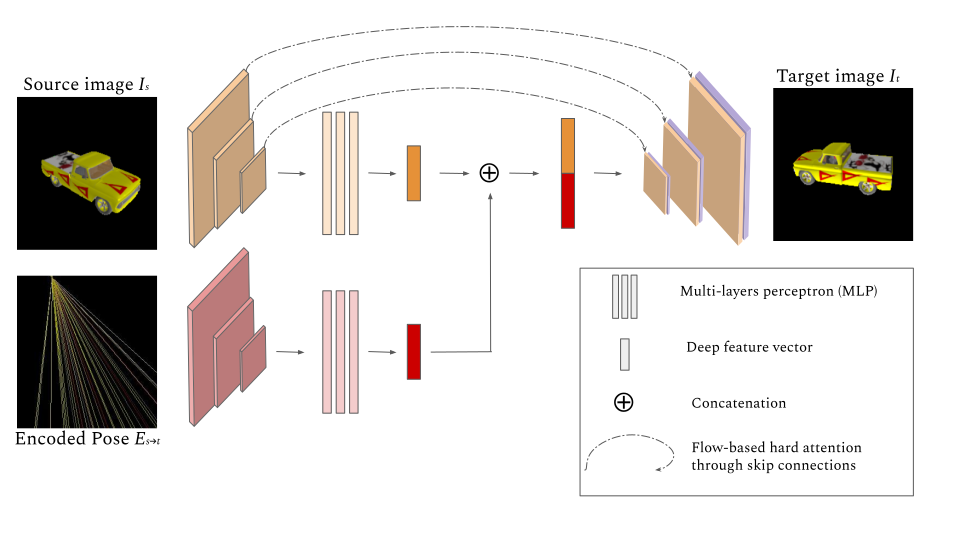
\includegraphics[width=\textwidth]{images/epipolarnvs/NetworkArchitecture.png}
  \end{center}
  \caption{\textbf{General overview of our architecture.} EpipolarNVS takes as inputs both $I_s$ and $E_{s\xrightarrow{}t}$ through two distinct encoders that produce feature vectors that are concatenated before being fed to the decoder. The neural network structure also leverages on the hard flow attention connections introduced in \citep{kim2020novel}.}
  \label{fig:architecture}
\end{figure}

Final loss function is a weighted sum  of a \ac{MAE}, referred as $\mathcal{L}_{1}$, and a second term, called $\mathcal{L}_{spectral}$, directly inspired by prior super-resolution work \citep{fritsche2019frequency}. This latter term extensively focuses on the preserving high frequencies components in the synthesized novel viewpoint. Considering a 2D Gaussian filter $w_{gauss}$, an image $I$ can be decomposed into a low and a high-frequency components, denoted as $I^{LF}$ and $I^{HF}$, respectively. 

\begin{equation}
\begin{cases}
     I^{LF}  = I\circledast w_{gauss} \\
     I^{HF} = I - I^{LF} = (\delta - w_{gauss})\circledast I
\end{cases}
\end{equation}
where $\circledast$ represents a 2D convolution operation. 

The final loss function used during training is thus given by: 
\begin{equation}
    \mathcal{L} = \mathcal{L}_{1} + \lambda \mathcal{L}_{spectral} = |\hat{I}_{t} - I_{t}| + \lambda \left( \hat{I}_{t}^{HF} - I_{t}^{HF} \right)^{2}
    \label{eq:1}
\end{equation}
 \newline

The Gaussian filter $w_{gauss}$ we used is straightforwardly defined by a mean $\mu = \frac{k_{s}-1}{2}$ and a variance $\sigma = (\frac{k_{s}}{k_{s}+1})^{2}$, with $k_{s}$=5.

This spectral term extensively focuses on the highest frequencies of the target and generated images, encouraging the network during training to recover as many fine and complex structures as possible.

\section{Experiments}
All qualitative and quantitative results we obtained through our camera pose encoding strategy are presented in this section. \newline

\noindent\textbf{Datasets.} We trained and tests our method on the \textit{chair} and \textit{car} classes from ShapeNet \citep{chang2015shapenet} as well as on real scene images from KITTI \citep{geiger2012we} and Synthia \citep{ros2016synthia}.
Results we reported for \citep{kim2020novel} slightly differ from the ones originally published by authors since we get consideration for a more challenging rendering scenario. We jittered camera pose in ShapeNet \citep{chang2015shapenet} and image borders from Synthia \citep{ros2016synthia} and KITTI \citep{geiger2012we} were not removed by center-cropping operation. Such changes are motivated and fully exposed in Appendix \ref{annex:epipolarnvs-dataset}.  \newline

\noindent\textbf{Training - Testing.} We trained our model on 100,000 iterations, using the same training procedure as \citep{kim2020novel}. Inference scores were averaged over 100 runs with batch size of 16. \newline

\noindent\textbf{Metrics.} We used the \ac{MAE},  \ac{SSIM} \citep{wang2004image} and \ac{PSNR} metrics to score our single-image \ac{NVS} architecture. 

\subsection{Qualitative Results}

Figure \ref{fig:res_all} presents instances from all the datasets we consider. While our model successfully infers and reasons about object size relative to the target view for the \textit{Car} and \textit{Chair} classes, the novel views produced by \citep{kim2020novel} fails to do so, generating results that roughly match the source object size. Our results on these two classes are also sharper and more realistic, both in term of colour and geometry. For instance, the car's wheels and the chair's intricate back are better synthesized using our method. 

Since \citep{kim2020novel} integrates the camera pose as discretized bins, the viewpoint transformation loses its physical 3D consistency. On the other hand, our method encodes the continuous pose transformation in a way that fully captures the underlying 3D structure.\newline


\begin{figure*}[h!]
    \begin{center}
    \includegraphics[width=\textwidth]{images/epipolarnvs/resultsFinal_BMVC.jpg}
    \end{center}
     \caption{\textbf{Novel view synthesis on the four considered datasets.} Encoded transformation $E_{s\xrightarrow{}t}$ have been obtained with $\textbf{G}_{15}$. From left to right: the source image  $I_s$, $E_{s\xrightarrow{}t}$, \citep{kim2020novel} prediction, our prediction, the target image $I_t$. On overall, our method predicts more consistent results since complete pose transformation has been fed to the network contrary to concurrent work \citep{kim2020novel}. }
     \label{fig:res_all}
\end{figure*}

The results of our method on real-world datasets are shown in the third (Synthia \citep{ros2016synthia}) and fourth (KITTI \citep{geiger2012we}) rows of Figure \ref{fig:res_all}. Notably, in the Synthia \citep{ros2016synthia} dataset, one can observe the car’s motion between the source and target views. While our results remain somewhat blurry, our network successfully hallucinated the forward motion of the bus. Our main concurrent work however replicates the source image and fails to capture the relative displacement in this example. A similar scenario is observed in the KITTI \citep{geiger2012we} dataset. While the sign "30" on the ground disappears between the two views, our method captures this drastic change,  whereas \citep{kim2020novel} stuggles as it did previously. We emphasise the role our camera encoding strategy plays here, especially regarding the shape of various objects where the perspective changes significantly between $I_s$ and $I_t$ (such as the roof of the house in the top-left corner). \newline


While results presented in Figure \ref{fig:res_all} for real world datasets highlight the overall motion that occurred, we focus in Figure \ref{fig:res_all2} on the extent to which high-frequency details are recovered by our model. Although the global motion is reasonably well handled by \citep{kim2020novel}, our method better retrieves tiny details, such as the paintings on the ground. The Spectral loss we used during training helped the network handle these high-frequency details. 

\begin{figure*}[h!]
    \begin{center}
    \includegraphics[width=\textwidth]{images/epipolarnvs/rebbutal_KITTI_3.jpg}
    \end{center}
     \caption{\textbf{Addional inference results on KITTI dataset.} From left to right: the source image  $I_s$, \citep{kim2020novel} prediction, our prediction, the target image $I_t$. Painting on the ground are better reconstructed in our method compared to \citep{kim2020novel}.}
     \label{fig:res_all2}
\end{figure*}

  
\subsection{Quantitative Results}

We present performance results across the four datasets we considered. Tables \ref{tab:1} and \ref{tab:2} respectively summarize the scores for the synthetic ShapeNet \citep{chang2015shapenet} dataset and the real-scene ones (Synthia \citep{ros2016synthia} and KITTI \citep{geiger2012we}). While our method outperforms concurrent approaches on the \ac{MAE} metric, we also achieve highly competitive results on SSIM, with only \citep{sun2018multiview} achieving better scores. \newline

We emphasise on an important aspect regarding the reported scores. Only our method and the one from \citep{kim2020novel} has been retrained with the extended and challenging datasets that we introduced earlier. Results from remaining works \citep{tatarchenko2015single,zhou2016view,park2017transformation,sun2018multiview,} are the original ones published by the respective authors. 

\begin{table}[h!]
    \caption{\textbf{Quantitative results.} Comparisons against state-of-the-art methods on the category specific \textit{Chairs} and \textit{Cars} classes from the ShapeNet dataset \citep{chang2015shapenet}. Best results are highlighted in \colorbox{red!25}{red}, second ones in \colorbox{orange!25}{orange} and third ones in \colorbox{yellow!25}{yellow}. }
    \label{tab:1}
    \begin{center}%\centering%
    \begin{adjustbox}{width = \linewidth}
    \begin{tabular}[h]{c||cccccccc}
    \hline
     Modality & Method & \multicolumn{3}{c}{Car} & \multicolumn{3}{c}{Chair} \\
     & &  MAE ($\downarrow$) & SSIM ($\uparrow$) & PSNR ($\uparrow$) & MAE ($\downarrow$) & SSIM ($\uparrow$) & PSNR ($\uparrow$)\\
    \hline
    Multi-view & \citep{sun2018multiview}& 0.078 & 0.935 & - & 0.141 & 0.911 & - \\
    \hline
     & \citep{tatarchenko2015single} & 0.139 & 0.875 & - & 0.223 & 0.882 & -\\
    &  \citep{zhou2016view} & 0.148 & 0.877 & - & 0.229 & 0.871 & - \\
    Single-view &  \citep{park2017transformation} & \cellcolor{yellow!25}0.119 & \cellcolor{orange!25}0.913 & - & \cellcolor{yellow!25}0.202 & \cellcolor{yellow!25}0.889& -\\
     &  \citep{yu2021pixelnerf} & - & \cellcolor{yellow!25}0.900 & \cellcolor{orange!25}23.17 & - & \cellcolor{red!25}0.911 & \cellcolor{red!25}23.72 \\
     &  \citep{kim2020novel} & \cellcolor{orange!25}0.026 & 0.892 & \cellcolor{yellow!25}21.18 & \cellcolor{orange!25}0.045 & 0.865 & \cellcolor{yellow!25}17.89 \\
     & Ours & \cellcolor{red!25}0.016 & \cellcolor{red!25}0.928 & \cellcolor{red!25}24.23 & \cellcolor{red!25}0.032 & \cellcolor{orange!25}0.901 & \cellcolor{orange!25}19.55 \\
     
    \hline 
    \end{tabular}
    \end{adjustbox}
    \end{center}
    \end{table}

 Results on the Synthia \citep{ros2016synthia} and KITTI \citep{geiger2012we} datasets are reported in Table \ref{tab:2}. Our model performance is competitive with current state of the art methods. We highlight that our method, as well as \citep{kim2020novel}, was trained on more complex scenarios from an image-content perspective: both Synthia and KITTI images were resized to $256\times 256$ without any center-cropping, which would have removed the most challenging elements from the scenes.

\begin{table}[h!]
    \caption{\textbf{Quantitative results.} Comparisons against state-of-the-art methods Synthia \citep{ros2016synthia} and KITTI \citep{geiger2012we} datasets. Best results are highlighted in \colorbox{red!25}{red}, second ones in \colorbox{orange!25}{orange} and third ones in \colorbox{yellow!25}{yellow}. }
    \label{tab:2}
    \begin{center}%\centering%
    \begin{adjustbox}{width = \linewidth}
    \begin{tabular}[h]{c||cccccccc}
    \hline
     Modality & Method & \multicolumn{3}{c}{Synthia} & \multicolumn{3}{c}{KITTI} \\
     & &  MAE ($\downarrow$) & SSIM ($\uparrow$) & PSNR ($\uparrow$) & MAE ($\downarrow$) & SSIM ($\uparrow$) & PSNR ($\uparrow$)\\
    \hline
    Multi-view & \citep{sun2018multiview}& 0.118 & 0.737 & - & 0.163 & 0.691 & - \\
    \hline
     & \citep{tatarchenko2015single} & \cellcolor{orange!25}0.175 & 0.612 & - & \cellcolor{yellow!25}0.295 & \cellcolor{yellow!25}0.505 & -\\
     Single-view &  \citep{zhou2016view} & \cellcolor{yellow!25}0.221 & \cellcolor{red!25}0.636 & - & 0.418 & 0.504 & - \\
     &  \citep{kim2020novel} & \cellcolor{red!25}0.065 & \cellcolor{orange!25}0.632 &  \cellcolor{red!25}19.81 & \cellcolor{orange!25}0.087 & \cellcolor{orange!25}0.602 & \cellcolor{orange!25}16.84 \\
     & Ours & \cellcolor{red!25}0.065 & \cellcolor{yellow!25}0.631 & \cellcolor{orange!25}19.44 & \cellcolor{red!25}0.082 & \cellcolor{red!25}0.609 & \cellcolor{red!25}17.11 \\
    \hline 
    \end{tabular}
    \end{adjustbox}
    \end{center}
    \end{table}

\subsection{Ablation studies}
\label{sec:ablation}
We conducted ablation studies to highlight and understand how key properties of our encoding strategy behave. \newline

\textbf{Benefit of the extended encoded pose strategy.}

Handling real-world datasets, where a maximum 10 frames can separate the source and the target views, represents a challenging configuration for single-image \ac{NVS}. Therefore, we conducted an intial ablation study to validate the intuition behind the additional channel that encodes the largest relative motion in the (XZ) plane. The spectral loss was not included during training in this ablation study, resulting in slighlty different outcomes from the originally reported results. 

\begin{table}[h!]
    \caption{\textbf{Ablation comparison.} Benefit on Synthia \citep{ros2016synthia} and KITTI \citep{geiger2012we} datasets of our extended encoding strategy. Adding such fourth channel helps the network to better perform on real-world datasets. The grid $\textbf{G}_{15}$ has been used in both cases. Best results are highlighted in \colorbox{red!25}{red}. }
    \label{tab:compExtended}
    \begin{center}%\centering%
    \begin{adjustbox}{width =.8\linewidth}
    \begin{tabular}[h]{c||ccccc}
    \hline
      Method & \multicolumn{2}{c}{Synthia} & \multicolumn{2}{c}{KITTI} \\
      &  MAE ($\downarrow$) & SSIM ($\uparrow$) & MAE ($\downarrow$) & SSIM ($\uparrow$) \\
    \hline
    3-\textit{channels} encoding & 0.077 & 0.602 & 0.109 & 0.576  \\
    4-\textit{channels} encoding & \cellcolor{red!25}0.066 & \cellcolor{red!25}0.622 & \cellcolor{red!25}0.086 & \cellcolor{red!25}0.605 \\
    \hline 
    \end{tabular}
    \end{adjustbox}
    \end{center}
    \end{table}

As shown in Table \ref{tab:compExtended}, and considering the neural network architecture as fixed, the fourth channel added to our representation $E_{s\xrightarrow{}t}$ clearly improves the network's performance on the task it was trained for. The SSIM increased by more than 2 points on average, while the \ac{MAE} significantly decreased (by almost 20\% on average across the two datasets), reaching competitive results compared to \cite{kim2020novel}. 

\begin{figure}[htp]

\begin{center}
\includegraphics[width=.45\textwidth]{images/epipolarnvs/ablationSynthia.png} \hfill
\includegraphics[width=.45\textwidth]{images/epipolarnvs/ablationSynthia2.png}
\end{center}
\caption{\textbf{Impact of a fourth channel into our encoding scheme.} Source fixed view $I_s$ (top row, Left) and three consecutive target views (bottom row, Left) from Synthia \cite{ros2016synthia} test set. - Predictions made by our model with the encoded pose (top row,Right) and the extended encoded pose strategy (bottom row,Right). Adding an additional channel in our extended pose encoding allows the network to better apprehend the motion that occurred in Synthia \cite{ros2016synthia} and KITTI \cite{geiger2012we}. The grid $\textbf{G}_{15}$ has been used in both cases.}
\label{fig:ablaSynthia}
\end{figure}

We highlight in Figure \ref{fig:ablaSynthia} the positive influence this additional channel has on the our model. While the manhole cover (which disappears in the target view sequence) is completely  ignored by the network trained with the three-channel pose encoding representation, the extended version we proposed successfully captures the car's motion.\newline 

\textbf{Spectral loss influence.}

A second ablation study was conducted to highlight the extent to which the spectral loss function positively impacts the training of our model architecture. 
\begin{table}[h!]
    \caption{\textbf{Ablation study.} Impact of the Spectral loss function over the four differerents datasets EpipolarNVS has been trained and tested on.}
    \label{tab:spectral}
\begin{center}
\begin{tabular}{@{}||lllllllllllllllll@{}}
  \toprule
  Datasets & Metrics  &$\mathcal{L}_{1}$ only  &  $\mathcal{L}_{1}+\mathcal{L}_{spectral}$ &   \\
  \midrule
  \multirow{3}{*}{ShapeNet - Car \citep{chang2015shapenet}} & MAE ($\downarrow$) &\hfil 0.019 & \hfil  \cellcolor{red!25}0.016 \\
  & SSIM ($\uparrow$) & \hfil0.912 & \hfil \cellcolor{red!25}0.928\\
  & PSNR ($\uparrow$)& \hfil22.61 & \hfil \cellcolor{red!25}24.23\\
  \midrule
  \multirow{3}{*}{ShapeNet - Chair \citep{chang2015shapenet}} & MAE ($\downarrow$) & \hfil 0.037 & \hfil \cellcolor{red!25}0.032\\
  & SSIM ($\uparrow$)&\hfil 0.892 & \hfil \cellcolor{red!25}0.901 \\
  & PSNR ($\uparrow$) & \hfil 19.19 & \hfil \cellcolor{red!25}19.55 \\
  \midrule
  \multirow{3}{*}{Synthia \citep{ros2016synthia}} & MAE ($\downarrow$)& \hfil 0.066 & \hfil \cellcolor{red!25}0.065\\
  & SSIM ($\uparrow$)& \hfil 0.622 & \hfil \cellcolor{red!25}0.631 \\
  & PSNR ($\uparrow$)& \hfil 19.24 & \hfil \cellcolor{red!25}19.44\\
  \midrule
  \multirow{3}{*}{KITTI \citep{geiger2012we}} & MAE ($\downarrow$)& \hfil 0.086 & \hfil \cellcolor{red!25}0.082\\
  & SSIM ($\uparrow$)& \hfil 0.605 & \hfil \cellcolor{red!25}0.609 \\
  & PSNR ($\uparrow$)& \hfil 16.99 & \hfil \cellcolor{red!25}17.11\\\hline

\end{tabular}
\end{center}
\end{table}

As shown in Table \ref{tab:spectral}, constraining the training to focus on high frequencies helps the network generate more realistic novel views. This quantitative improvement is visually confirmed in Figure \ref{fig:spectral_res}, where the same object instance is generated using both configurations from the ShapeNet \textit{Car} class.\newline 

\begin{figure*}[h!]
    \begin{center}
    \includegraphics[width=\textwidth]{images/epipolarnvs/spectralCar.jpg}
    \end{center}
     \caption{Inference results from the ShapeNet ~\cite{chang2015shapenet} \textit{Car} test set. From the top row to the bottom one: Source images  $I_s$, Ours prediction with $\mathcal{L}_{1}$ only at training, Ours prediction with  $\mathcal{L}_{spectral} + \mathcal{L}_{1}$ at training, Ground truth - Target images $I_t$. From a general perspective, tires and windows are better retrieved at inference time when high frequencies have been constrained during training.}
     \label{fig:spectral_res}
\end{figure*}

\textbf{Discrete grid $\textbf{G}_{r}$ granularity and sampling strategy.}

We present a third ablation study to gain insight into the granularity required for our grid sampling. In addition to the three grids we tested, we also consider a random sampling strategy, which involves sampling a fixed number of locations (corresponding to 1\% of the pixels for a $256\times 256$ image) of locations. Table \ref{tab:3} summarizes the results of this experiment on the real-world datasets.

\begin{table}[h!]
    \caption{\textbf{Ablation comparison.} Sampling strategy influence over the real-world datasets Synthia \citep{ros2016synthia} and KITTI \citep{geiger2012we}. Best results are highlighted in \colorbox{red!25}{red}. }
    \label{tab:3}
    \begin{center}%\centering%
    \begin{adjustbox}{width =\linewidth}
    \begin{tabular}[h]{c||ccccc}
    \hline
      Method & \multicolumn{2}{c}{Synthia} & \multicolumn{2}{c}{KITTI} \\
      &  MAE ($\downarrow$) & SSIM ($\uparrow$) & MAE ($\downarrow$) & SSIM ($\uparrow$) \\
    \hline
    \makecell{ Random Sampling \\ \footnotesize{(655 pix. sampled)}}& \cellcolor{red!25}0.0816 & \cellcolor{red!25}0.593 & 0.1290 & 0.549   \\ \hline
\makecell{$\textbf{G}_{15}$ grid \\ \footnotesize{(225 pix. sampled)}} & 0.0823 & 0.589 & 0.1222 & 0.562   \\ \hline
\makecell{$\textbf{G}_{20}$ grid \\ \footnotesize{(400 pix. sampled)}} & 0.0857 & 0.576 & 0.1241 & 0.560  \\ \hline
\makecell{$\textbf{G}_{25}$ grid \\ \footnotesize{(625 pix. sampled)}} & 0.0908 & 0.575 & \cellcolor{red!25}0.1217 & \cellcolor{red!25}0.563   \\ 
    \hline 
    \end{tabular}
    \end{adjustbox}
    \end{center}
    \end{table}


Overall, there are no significant differences between the strategies tested in this ablation study.  However, the random and grid sampling strategies differ in one important aspect: the latter performs significantly faster, taking roughly four times less time to form a batch of triplets $\left(I_{s},I_{t},E_{s\xrightarrow{}t}\right)$ than the random sampling strategy. \newline

Using a regular grid $\textbf{G}_{r}$ always samples the same pixel locations from $I_s$ to build  $E_{s\xrightarrow{}t}$, while the random sampling strategy requires new samples to be picked each time.  

We performed the same ablation study on the synthetic ShapeNet dataset ~\cite{chang2015shapenet} and observed identical observations.

\section{Limitations and further works}
The pose encoding strategy introduced in this chapter is an innovative solution for integrating camera pose transformations in into the \ac{NVS} problem. However, our method has some limitations that could be addressed to achieve better results in both image quality and processing speed. Since we compute the encoded viewpoint transformation $E_{s\xrightarrow{}t}$ \textit{on the fly} during training, our method is slower than the main concurrent work \citep{kim2020novel} to ours. Another potential improvement lies in making the camera data requirements more flexible, as our method currently requires both intrinsic and extrinsic parameters. 

Finally, future work could explore leveraging the encoded relative poses we designed to better constrain the network during training by using a cyclic loss function. Specifically, it would be possible to define a reversed encoded relative pose, $E_{t\xrightarrow{}s}$, by leveraging the predicted novel view. 

\section{Conclusion}
In this chapter, we introduced a novel method for encoding camera transformations for learning-based \ac{NVS}. Our approach leverages epipolar geometry to encode viewpoint displacement as an image, which we refer to as the encoded relative pose $E_{s\xrightarrow{}t}$ (composed of several colored epipolar lines). We argue that this new camera transformation encoding is better suited for the single-image \ac{NVS} task than the standard approach, which considers only the extrinsic camera transformation. The traditional method involves feeding the neural network with an RGB source image and a camera viewpoint transformation to generate a new image that reflects the impact of the displacement on the input image. Instead, our method provides both an RGB source image and an encoded image of the viewpoint transformation, offering a stronger insight into the effect of the displacement. In other words, the core motivation behind our method is to help the network better understand the correlation between the input image and the desired camera viewpoint transformation. The experimental results across various datasets presented in this work support our claim. These results demonstrate that this new encoding strategy is more robust to complex displacements, such as large perspective changes, and also produces images with sharper details.